\documentclass{beamer}
\usetheme{Madrid}
\usecolortheme{default}
\usepackage{tikz}
\usepackage{amsmath, amssymb, amsthm}

\title{Applications of Linear Algebra}
\author{Muhammed Shameel}
\date{\today}

\begin{document}

\frame{\titlepage}

\begin{frame}{Table of Contents}
    \tableofcontents
\end{frame}

\section{Introduction}

\begin{frame}{Introduction}
    A \textbf{vector space} $V$ over a field $F$ (e.g., $\mathbb{R}, \mathbb{C}, \mathbb{Q}$) is a set of vectors satisfying given axioms under addition and scalar multiplication:
    \begin{enumerate}
        \item \textbf{Addition:} Must be associative, commutative, have an identity ($\mathbf{0}$), and have inverses ($-\mathbf{v}$).
        \item \textbf{Scalar Multiplication:} Defines how a scalar $c \in F$ scales a vector $\mathbf{v} \in V$. It must satisfy:
              \begin{itemize}
                  \item \textbf{Identity:} $1\mathbf{v} = \mathbf{v}$ for the multiplicative identity $1 \in F$.
                  \item \textbf{Compatibility:} $a(b\mathbf{v}) = (ab)\mathbf{v}$ for all $a, b \in F$.
                  \item \textbf{Distributivity over Vector Addition:} $a(\mathbf{u} + \mathbf{v}) = a\mathbf{u} + a\mathbf{v}$.
                  \item \textbf{Distributivity over Scalar Addition:} $(a + b)\mathbf{v} = a\mathbf{v} + b\mathbf{v}$.
              \end{itemize}
    \end{enumerate}
\end{frame}

\begin{frame}{Introduction (Examples)}
    \textbf{Examples:}
    \begin{itemize}
        \item \textbf{Polynomials:} $\mathbb{R}[x]$, the set of polynomials over $\mathbb{R}$
        \item \textbf{Matrices:} $M_{m \times n}(F)$, the set of all $m \times n$ matrices.
        \item \textbf{Function Spaces:} $C[a, b]$, the set of continuous real-valued functions on an interval.
    \end{itemize}
\end{frame}

\subsection{Basis and Dimension}
\begin{frame}{Basis and Dimension}
    A \textbf{basis} $\mathcal{B} = \{\mathbf{v}_1, \dots, \mathbf{v}_n\}$ for $V$ is a set that is:
    \begin{enumerate}
        \item \textbf{Linearly Independent:} $\sum c_i \mathbf{v}_i = \mathbf{0} \implies c_i = 0$ for all $i$.
        \item \textbf{Spanning:} Every $\mathbf{v} \in V$ is a linear combination of $\mathcal{B}$.
    \end{enumerate}
    \vfill
    Size of the basis is called \textbf{dimension} of $V$.
\end{frame}

\subsection{Eigenvalues and Eigenvectors}
\begin{frame}{Eigenvalues and Eigenvectors}
    For a square matrix $A \in M_{n \times n}(F)$, a non-zero vector $\mathbf{v}$ is an \textbf{eigenvector} if:
    \[A\mathbf{v} = \lambda\mathbf{v}\]
    where $\lambda \in F$ is the corresponding \textbf{eigenvalue}.

    \vfill

    This is equivalent to $(A - \lambda I)\mathbf{v} = \mathbf{0}$. For a non-zero solution to exist, the matrix $(A - \lambda I)$ must be singular, leading to the \textbf{characteristic equation}:
    \[\det(A - \lambda I) = 0\]
    where $I$ is the $n \times n$ identity matrix. The determinant yields a polynomial $p(\lambda)$ of degree $n$, whose roots are the eigenvalues of $A$.
\end{frame}

\section{Graph theory}
\begin{frame}{Graph theory}
    Graph theory is the study of graphs, which are mathematical structures used to model pairwise relations between objects.
    \vfill
    A \textbf{graph} $G = (V, E)$ consists of:
    \begin{itemize}
        \item \textbf{Vertices:} A set $V = \{v_1, v_2, \dots, v_n\}$ representing the objects.
        \item \textbf{Edges:} A set $E$ of pairs of vertices representing the connections between them.
    \end{itemize}
\end{frame}

\begin{frame}{Definitions}
    \begin{itemize}
        \item \textbf{Degree:} The degree of a vertex $v$, denoted $d(v)$, is the number of edges incident to it.
        \item \textbf{Walk:} A sequence of vertices and edges $v_0, e_1, v_1, e_2, \dots, e_k, v_k$ starting and ending at vertices.
        \item \textbf{Trail:} A walk in which no edges are repeated.
        \item \textbf{Path:} A walk in which no vertices (and consequently no edges) are repeated.
        \item \textbf{Connectedness:} A graph is \textbf{connected} if there is a path between every pair of vertices. A graph that is not connected is called \textbf{disconnected}.
        \item \textbf{Connected Component:} A maximal connected subgraph of a graph. Every graph can be uniquely partitioned into its connected components.
    \end{itemize}
\end{frame}

\begin{frame}{Special Graphs}
    \begin{itemize}
        \item \textbf{Complete Graph ($K_n$):} A graph where every pair of distinct vertices is connected by a unique edge. It has $\binom{n}{2}$ edges.
        \item \textbf{Bipartite Graph:} A graph whose vertices can be partitioned into two disjoint sets $U$ and $V$ such that every edge connects a vertex in $U$ to one in $V$. A \textbf{complete bipartite graph} $K_{m,n}$ contains all possible edges between the two sets.
        \item \textbf{Tree:} A connected graph that contains no cycles. For a graph with $n$ vertices, being a tree is equivalent to being connected and having exactly $n-1$ edges.
    \end{itemize}
\end{frame}

\subsection{Adjacency Matrix}
\begin{frame}[fragile]{Adjacency Matrix}
    The \textbf{adjacency matrix} $A$ of a graph $G$ with $n$ vertices is an $n \times n$ matrix where the entry $a_{ij}$ is defined as:
    \[a_{ij} = \begin{cases} 1 & \text{if there is an edge between } v_i \text{ and } v_j \\ 0 & \text{otherwise} \end{cases}\]
    \vfill
    \textbf{Example:}
    $V = \{v_1, v_2, v_3, v_4\}$, $E = \{(v_1, v_2), (v_1, v_3), (v_2, v_3), (v_3, v_4)\}$
    \begin{columns}
        \begin{column}{0.4\textwidth}
            \begin{center}
                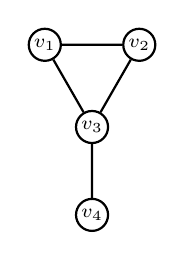
\begin{tikzpicture}[scale=1.2,thick,every node/.style={circle,draw,minimum size=0.3cm,inner sep=1pt}]
                    \node (v1) at (0,1) {\scriptsize $v_1$};
                    \node (v2) at (1,1) {\scriptsize $v_2$};
                    \node (v3) at (0.5,0.13) {\scriptsize $v_3$};
                    \node (v4) at (0.5,-0.8) {\scriptsize $v_4$};
                    \draw (v1) -- (v2);
                    \draw (v2) -- (v3);
                    \draw (v1) -- (v3);
                    \draw (v3) -- (v4);
                \end{tikzpicture}
            \end{center}
        \end{column}
        \begin{column}{0.6\textwidth}
            \[A = \begin{pmatrix} 0 & 1 & 1 & 0 \\ 1 & 0 & 1 & 0 \\ 1 & 1 & 0 & 1 \\ 0 & 0 & 1 & 0 \end{pmatrix}\]
        \end{column}
    \end{columns}
\end{frame}


\begin{frame}{Remarks}
    \begin{itemize}
        \item \textbf{Symmetry:} For an undirected graph, the adjacency matrix is symmetric ($A = A^T$).
        \item \textbf{Vertex Degree:} The sum of the entries in the $i$-th row (or column) of $A$ is equal to the degree $d(v_i)$ of the vertex $v_i$.
    \end{itemize}
\end{frame}

\begin{frame}{Powers of the Adjacency Matrix}
    \textbf{Theorem:} Let $A$ be the adjacency matrix of a graph $G$. The entry $(A^k)_{ij}$ is equal to the number of walks of length $k$ from vertex $v_i$ to vertex $v_j$.
    \vfill
    \textbf{Corollary:} The number of triangles in a simple graph $G$ is given by:
    \[ \text{Number of triangles} = \frac{1}{6} \text{tr}(A^3) \]
    where $\text{tr}(A^3)$ is the trace of $A^3$. (Walks of length 3 starting/ending at $v_i$ must be triangles; each counted 6 times due to 3 vertices and 2 directions).
\end{frame}
\begin{frame}{}
\end{frame}
\subsection{Matchings}
\begin{frame}{Matchings}
    A \textbf{matching} $M$ in a graph $G = (V, E)$ is a subset of edges s.t. no two edges share a common vertex.
    \vfill
    A \textbf{perfect matching} covers all vertices. $M$ is perfect if every $v \in V$ is incident to exactly one edge in $M$. $|V|$ must be even, and matching contains $|V|/2$ edges.
\end{frame}

\subsection{Adjacency Matrix of Bipartite Graphs}
\begin{frame}{Adjacency Matrix of Bipartite Graphs}
    If $G$ is bipartite with vertex partitions $U$ and $V$ of size $m$ and $n$, block form:
    \[A = \begin{pmatrix} \mathbf{0}_{m \times m} & B \\ B^T & \mathbf{0}_{n \times n} \end{pmatrix}\]
    where $b_{ij} = 1$ if edge between $u_i \in U$ and $v_j \in V$, and $0$ otherwise.
    \vfill
    \textbf{Theorem:} For partitions $U, V$ of equal size $n$, $G$ has a perfect matching iff $\det(B) \neq 0$.
\end{frame}

\begin{frame}{Leibniz Formula}
    \textbf{Lemma (Leibniz Formula):}
    \[\det(B) = \sum_{\sigma \in S_n} \text{sgn}(\sigma) \prod_{i=1}^n b_{i, \sigma(i)}\]
    \vfill
    \textbf{Proof of Lemma:}
    $\det(B) = \det\left(\sum_{j_1=1}^n b_{1,j_1} \mathbf{e}_{j_1}, \dots, \sum_{j_n=1}^n b_{n,j_n} \mathbf{e}_{j_n}\right)$
    \[ = \sum_{j_1, \dots, j_n} \left( \prod_{i=1}^n b_{i,j_i} \right) \det(\mathbf{e}_{j_1}, \dots, \mathbf{e}_{j_n}) \]
\end{frame}
\begin{frame}{}
\end{frame}

\subsection{Incidence Matrix}
\begin{frame}[fragile]{Incidence Matrix}
    To define the \textbf{incidence matrix} $Q$, we assign an arbitrary direction to each edge $e_j$. The entries of $Q$ are:
    \[q_{ij} = \begin{cases} -1 & \text{if } v_i \text{ is source of } e_j \\ 1 & \text{if } v_i \text{ is target of } e_j \\ 0 & \text{otherwise} \end{cases}\]
    \vfill
    \textbf{Example:} $e_1: v_1 \to v_2$, $e_2: v_1 \to v_3$, $e_3: v_2 \to v_3$, $e_4: v_3 \to v_4$:
    \begin{columns}
        \begin{column}{0.4\textwidth}
            \begin{center}
                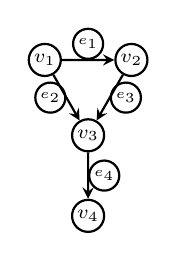
\begin{tikzpicture}[scale=1.1,thick,every node/.style={circle,draw,minimum size=0.3cm,inner sep=1pt}]
                    \node (v1) at (0,1) {\scriptsize $v_1$};
                    \node (v2) at (1,1) {\scriptsize $v_2$};
                    \node (v3) at (0.5,0.13) {\scriptsize $v_3$};
                    \node (v4) at (0.5,-0.8) {\scriptsize $v_4$};
                    \draw[->,>=stealth] (v1) -- (v2) node[midway, above] {\tiny $e_1$};
                    \draw[->,>=stealth] (v1) -- (v3) node[midway, left] {\tiny $e_2$};
                    \draw[->,>=stealth] (v2) -- (v3) node[midway, right] {\tiny $e_3$};
                    \draw[->,>=stealth] (v3) -- (v4) node[midway, right] {\tiny $e_4$};
                \end{tikzpicture}
            \end{center}
        \end{column}
        \begin{column}{0.6\textwidth}
            \[Q = \begin{pmatrix} -1 & -1 & 0 & 0 \\ 1 & 0 & -1 & 0 \\ 0 & 1 & 1 & -1 \\ 0 & 0 & 0 & 1 \end{pmatrix}\]
        \end{column}
    \end{columns}
\end{frame}

\begin{frame}{Incidence Matrix Rank}
    \textbf{Lemma:} For a connected graph $G$ with $n$ vertices, $\text{rank}(Q) = n-1$.
    \vfill
    \textbf{Proof Sketch:}
    \vspace{2cm}
\end{frame}

\begin{frame}{Incidence Matrix Rank}
    \textbf{Theorem:} If $G$ is a graph on $n$ vertices and has $k$ connected components, then $\text{rank}(Q(G)) = n - k$.
    \vfill
    \textbf{Corollary:} The dimension of the null space of $Q(G)$ is equal to the number of connected components $k$.
\end{frame}
\begin{frame}{}
\end{frame}

\section{Polynomials}
\begin{frame}{Polynomials}
    The set of all polynomials over $\mathbb{F}$, $\mathcal{P}$, forms an infinite-dimensional vector space.
    $\mathcal{P}_n$ (degree at most $n$) is a subspace.
    \vfill
    \textbf{Standard Basis for $\mathcal{P}_n$:}
    $\mathcal{B} = \{1, x, x^2, \dots, x^n\}$
    $\dim(\mathcal{P}_n) = n+1$.
\end{frame}

\subsection{Polynomial Interpolation}
\begin{frame}{Polynomial Interpolation}
    \textbf{Problem:} Given $n+1$ distinct points $(x_i, y_i)$, does there exist a unique $p(x) \in \mathcal{P}_n$ s.t. $p(x_i) = y_i$?
    \[
        \begin{cases}
            a_0 + a_1 x_0 + \dots + a_n x_0^n = y_0 \\
            \vdots                                  \\
            a_0 + a_1 x_n + \dots + a_n x_n^n = y_n
        \end{cases}
    \]
    Matrix form: $V\mathbf{a} = \mathbf{y}$ where $V$ is the \textbf{Vandermonde matrix}:
    \[ \begin{pmatrix} 1 & x_0 & \dots & x_0^n \\ \vdots & \vdots & \ddots & \vdots \\ 1 & x_n & \dots & x_n^n \end{pmatrix} \begin{pmatrix} a_0 \\ \vdots \\ a_n \end{pmatrix} = \begin{pmatrix} y_0 \\ \vdots \\ y_n \end{pmatrix} \]
    Since $x_i$ are distinct, $\det(V) = \prod_{0 \le i < j \le n} (x_j - x_i) \neq 0$.
\end{frame}

\begin{frame}{Lagrange Basis}
    We look for a different basis for $\mathcal{P}_n$ that simplifies the interpolation problem. Given $n+1$ distinct points $x_0, x_1, \dots, x_n$, the \textbf{Lagrange basis} $\{L_0(x), L_1(x), \dots, L_n(x)\}$ is defined such that:
    \[L_j(x_i) = \delta_{ij} = \begin{cases} 1 & \text{if } i = j \\ 0 & \text{if } i \neq j \end{cases}\]

    The basis polynomials are given by:
    \[L_j(x) = \prod_{\substack{0 \le i \le n \\ i \neq j}} \frac{x - x_i}{x_j - x_i}\]
\end{frame}

\begin{frame}{Lagrange Interpolation}
    In this basis, the unique interpolating polynomial $p(x)$ is simply:
    \[p(x) = \sum_{j=0}^n y_j L_j(x)\]

    \textbf{Remark:} In the Lagrange basis, the matrix representation of the interpolation problem $V\mathbf{a} = \mathbf{y}$ becomes the identity matrix $I$, as the coefficients of $p(x)$ are exactly the values $y_j$.
\end{frame}
\begin{frame}{}
\end{frame}

\subsection{Resultant and Sylvester Matrix}
\begin{frame}{Resultant and Sylvester Matrix}
    The \textbf{resultant} of $p(x), q(x)$ determines if they share a common root.
    $p(x) = \sum_{i=0}^n a_i x^i$, $q(x) = \sum_{j=0}^m b_j x^j$.
    The \textbf{Sylvester matrix} $S(p, q)$ is an $(n+m) \times (n+m)$ matrix:
    \[ S(p, q) = \begin{pmatrix} a_n & \dots & a_0 & 0 & \dots \\ 0 & a_n & \dots & a_0 & \dots \\ \vdots & \vdots & \ddots & \vdots & \ddots \\ b_m & \dots & b_0 & 0 & \dots \\ \vdots & \vdots & \ddots & \vdots & \ddots \end{pmatrix} \]
\end{frame}

\begin{frame}{Resultant Properties}
    \textbf{Resultant:} $\text{res}(p, q) = \det(S(p, q))$. If $\neq 0$, no common roots.
    \vfill
    If $\deg(p)=n, \deg(q)=m$, then $\gcd(p,q) \neq 0$ iff $q'p - p'q \equiv 0$ ($\deg(q')\le m-1, \deg(p')\le n-1$).
    \vfill
    Matrix equation:
    \[ S(p, q)^T \begin{pmatrix} q'_{m-1} \\ \vdots \\ -p'_{n-1} \\ \vdots \end{pmatrix} = \mathbf{0} \]
    Solutions exist iff $\det(S(p, q)) = 0$.
\end{frame}

\begin{frame}{Repeated Roots and Discriminant}
    Repeated root $\iff p(x)$ and $p'(x)$ share a root.
    \[ p(x) \text{ has repeated root} \iff \text{res}(p, p') = 0 \]
    Basis for the \textbf{discriminant} $\Delta(p) \propto \text{res}(p, p')$.
\end{frame}

\subsection{Algebraic Numbers}
\begin{frame}{Algebraic Numbers}
    A complex number $\alpha$ is called an \textbf{algebraic number} if it is a root of a non-zero polynomial with coefficients in $\mathbb{Q}$. That is, there exists $p(x) = a_nx^n + a_{n-1}x^{n-1} + \dots + a_0$ where $a_i \in \mathbb{Q}$ and $a_n \neq 0$, such that $p(\alpha) = 0$.

    \vfill

    \textbf{Problem:} Is the set of algebraic numbers $\overline{\mathbb{Q}}$ a field? \\
    i.e. given $\alpha, \beta \in \overline{\mathbb{Q}}$ does it have:
    \begin{itemize}
        \item \textbf{Addition}: $\alpha + \beta \in \overline{\mathbb{Q}}$
        \item \textbf{Additive Inverse}: $-\alpha \in \overline{\mathbb{Q}}$
        \item \textbf{Multiplication}: $\alpha \beta \in \overline{\mathbb{Q}}$
        \item \textbf{Multiplicative Inverse}: $1 / \beta \in \overline{\mathbb{Q}}$ (for $\beta \neq 0$)
    \end{itemize}
\end{frame}

\begin{frame}{Algebraic Numbers (Inverses)}
    The existence of inverses is straightforward:
    \begin{itemize}
        \item \textbf{Additive Inverse:} If $p(\alpha) = 0$, then $-\alpha$ is a root of $q(x) = p(-x) \in \mathbb{Q}[x]$.
        \item \textbf{Multiplicative Inverse:} If $p(\alpha) = 0$ for $\alpha \neq 0$, then $1/\alpha$ is a root of the reciprocal polynomial $q(x) = x^{\deg p} p(1/x) \in \mathbb{Q}[x]$.
    \end{itemize}
\end{frame}

\begin{frame}{Algebraic Numbers (Addition and Multiplication)}
    Given 2 polynomials $p(x), q(x)$, with roots $\alpha, \beta$ respectively we can use the resultant to find polynomials $r(x), s(x)$ with roots $\alpha + \beta, \alpha\beta$ respectively.
    \begin{align*}
        r(x) & = \text{res}_{y}\left(p(y),\text{res}_{z}(q(z),x-y-z)\right) \\
        s(x) & = \text{res}_{y}(p(y),\text{res}_{z}(q(z),x-yz))
    \end{align*}
    See that $\text{res}_{z}(q(z),x-y-z)$ becomes 0 when $x-y = \beta$, hence it is a polynomial in $y$ with $x-\beta$ as a root. Hence $r(x)$ becomes zero when $\alpha = x- \beta$, i.e $x = \alpha + \beta$.
\end{frame}

\section{Geometry}
\subsection{Euclidean distances}
\begin{frame}{Euclidean distances}
    Embeddability of $P_1, P_2, P_3$ with $d_{ij}$ in $\mathbb{R}^2$.
    \vfill
    Necessary/Sufficient: \textbf{Triangle inequality} $d_{ij} \le d_{ik} + d_{kj}$.
    \vfill
    \textbf{Example:} distance 1, 1, 3. No, as $3 \le 1+1=2$ is False.
    \vfill
    \textbf{Sufficiency Construction:} Intersecting circles $\mathcal{C}_1, \mathcal{C}_2$ at $P_1, P_2$ with radii $d_{13}, d_{23}$. Cross iff:
    \[ |d_{13} - d_{23}| \le d_{12} \le d_{13} + d_{23} \]
\end{frame}

\begin{frame}[fragile]{General case for $n$ points}
    Triangle inequality is necessary but not sufficient for $n>3$.
    \begin{center}
        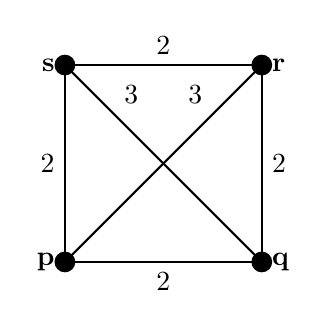
\begin{tikzpicture}[scale=2.5,thick]
            \coordinate (s) at (0,1);
            \coordinate (r) at (1,1);
            \coordinate (p) at (0,0);
            \coordinate (q) at (1,0);
            \draw (s) -- (r) node[midway, above] {2};
            \draw (p) -- (q) node[midway, below] {2};
            \draw (s) -- (p) node[midway, left] {2};
            \draw (r) -- (q) node[midway, right] {2};
            \draw (s) -- (q) node[pos=0.25, above right] {3};
            \draw (p) -- (r) node[pos=0.75, above left] {3};
            \foreach \n/\pos in {s/left, r/right, p/left, q/right}
            \fill (\n) circle (1.5pt) node[\pos] {$\mathbf{\n}$};
        \end{tikzpicture}
    \end{center}
    Subsets satisfy T.I., but four points cannot be embedded in $\mathbb{R}^k$.
\end{frame}

\begin{frame}{PSD Definition and Fact}
    $M \in \mathbb{R}^{n \times n}$ is \textbf{positive semi-definite (PSD)} if $x^T M x \ge 0$ for all $x$.
    \vfill
    \textbf{Fact:} A symmetric matrix $A$ is PSD iff $\exists X$ s.t. $A = X^T X$.
\end{frame}


\begin{frame}{Gram Matrix}
    \textbf{Theorem.} Let $m_{ij} \ge 0, i, j = 0, \dots, n$, with $m_{ij} = m_{ji}$ and $m_{ii} = 0$.
    Then points $\mathbf{p}_i \in \mathbb{R}^n$ with $\|\mathbf{p}_i - \mathbf{p}_j\| = m_{ij}$ exist iff $G$ with:
    \[ g_{ij} = \frac{1}{2}(m_{0i}^2 + m_{0j}^2 - m_{ij}^2) \]
    is positive semi-definite.
\end{frame}
\begin{frame}{}
\end{frame}
\subsection{Squaring a rectangle}
\begin{frame}[fragile]{Squaring a rectangle}
    \begin{center}
        \begin{tikzpicture}[scale=1.5]
            \draw (0,0) -- (2.5,0) node[midway, below] {$x$}
            -- (2.5,1) node[midway, right] {}
            -- (0,1) node[midway, above] {}
            -- (0,0) node[midway, left] {$1$};
            \draw (0,0) rectangle (2.5,1);
        \end{tikzpicture}
    \end{center}
    Problem: When can $1 \times x$ be tiled by finitely many squares?
    \vfill
    $x \in \mathbb{Q}$ ($x=p/q$): Tile with $pq$ squares of side $1/q$.
    \vfill
    \textbf{Theorem.} Irrational $x \implies$ cannot be tiled.
\end{frame}
\begin{frame}{}
\end{frame}

\begin{frame}[fragile]{Tiling Example}
    \begin{center}
        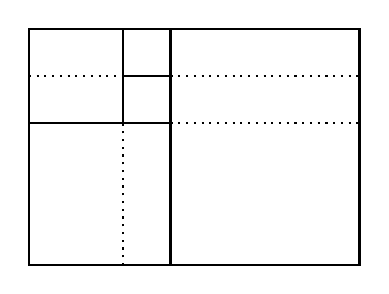
\begin{tikzpicture}[x=0.6cm, y=0.6cm, thick]
            \draw (0,0) rectangle (7, 5);
            \draw (3, 0) -- (3, 5);
            \draw (0, 3) -- (3, 3);
            \draw (2, 3) -- (2, 5);
            \draw (2, 4) -- (3, 4);
            \begin{scope}[dotted]
                \draw (2, 0) -- (2, 3);
                \draw (0, 4) -- (2, 4);
                \draw (3, 4) -- (7, 4);
                \draw (3, 3) -- (7, 3);
            \end{scope}
        \end{tikzpicture}
    \end{center}
\end{frame}

\end{document}
